\chapter{Fundamentação}\label{ch:Fundamentacao}

A fundamentação teórica é um elemento crucial para a compreensão dos fundamentos teóricos que dão base aos conceitos que permeiam o objeto de estudo em uma determinada pesquisa. O capítulo de fundamentação surge então para munir o pesquisador dos conhecimentos necessários para o andamento e a conclusão de sua pesquisa. Ao mesmo tempo, a fundamentação auxilia outros pesquisadores na idenficação das bases do conhecimento teórico que guiaram determinando estudo. 

O corrente estudo tem como cerne a validação de um programa educacional para a prevenção da violência sexual infantil baseado na dinâmicas de jogos sérios. Deste modo, a seção \ref{sec:JogosSerios} fundamenta o conceito de Jogos Sérios. A seção \ref{sec:Engenharia} trás alguns conceitos sobre o desenvolvimento de jogos. % A seção 2.3 discutei os sistemas de aplicação de programas educacionais e suas formas de validação. 

\vspace{0.75cm}

\section{Jogos Sérios}\label{sec:JogosSerios}

O termo \underline{Jo}g\underline{o Sério} (em inglês: \textit{Serious Game}) surge pela primeira vez na história em 1970 \cite{clark1970serious}. Desde então, o termo passou por inúmeras revisões até alcançar uma definição geral, a qual classifica como Jogo Sério: todos os jogos projetados para uma finalidade principal que não a pura diversão \cite{michael2005serious, de2015aprendizagem, laamarti2014overview}.

A definição geral de Jogos Sérios permite identificar que os jogos classificados como sérios antecedem a própria origem do termo. Isso pois, a história conta que antes da década de 70, alguns jogos já eram utilizados para outros propósitos além do entreterimento \cite{wilkinson2016brief}. Salienta-se no entanto que o termo não encontra-se verdadeiramente consolidado na literatura científica da área, existindo inclusive várias definições e termos correlatos \cite{pourabdollahian2012serious}.

Para definir melhor o termo \underline{Jo}g\underline{o Sério} que fundamentará e guiará o andamentamento do presente estudo, buscou-se separar o conceito e interpretar individualmente as palavras que o compõem. O termo \underline{Jo}g\underline{o} demarca o conjunto de atividades regidas por uma estrutura de regras focadas na diversão e no entreterimento \cite{kishimoto1994jogo}. Já o termo \underline{Sério} define um propósito prático a este conjunto de atividades, geralmente sendo pedagógico ou motor \cite{schroeder2017wobu, baptista2017jogos}. %(com os Exergames = Jogos Ativos). 
A Figura \ref{fig:JS}, ilustra de forma resumida os conceitos que fundamentam a definição de \underline{Jo}g\underline{o Sério} do atual trabalho.  

%Jogo: “é uma atividade mais estruturada e estabelecida por um princípio de regras mais explícitas” que integra tanto o objeto quanto a brincadeira (Kishimoto, 1994) ou “ação de jogar” (Bertoldo & others, 2000) %https://repositorio-aberto.up.pt/bitstream/10216/110820/2/253022.pdf

%Um game é uma atividade lúdica composta por uma série de ações e decisões, limitado por regras e pelo universo do game, que resultam em uma condição final. As regras e o universo do game são apresentados por meios eletrônicos e controlados por um programa digital (...) [e] existem para proporcionar uma estrutura e um contexto para as ações de um jogador. As regras também existem para criar situações interessantes com o objetivo de desafiar e se contrapor ao jogador. Jogos Sérios são aplicações que mesclam aspectos sérios como o ensino, a aprendizagem, a comunicação e a informação, com o lúdico e interativo fornecido pelos games, sendo o principal objetivo outro além do puro entretenimento. Criar um Jogo Sério é conseguir fundir de forma atraente e interessante informações para ensino, com interações dinâmicas e lúdicas (BOYLE; CONNOLLY; HAINEY, 2011, p. 71).%https://www.udesc.br/arquivos/cct/id_cpmenu/1024/diego_buchinger__1__15167055468902_1024.pdf

%Esta combinação tem como propósito tornar o conteúdoprático, útil (sério) e jogável, o que é alcançado por meio do desenvolvimento decenários que são ao mesmo tempo práticos e agradáveis.%https://webcache.googleusercontent.com/search?q=cache:fWC_TzjZ76QJ:https://www.br-ie.org/pub/index.php/pie/article/download/6595/4506+&cd=1&hl=pt-BR&ct=clnk&gl=br

%computer application, for which the original intention is to combine with consistency, both serious (Serious) aspects such as non-exhaustive and non-exclusive, teaching, learning, communication, or the information, with playful springs from the video game (Game). %http://hayka-kultura.org/images/Proceedings%20SGS%20Wkshp%202011%20ind%2004.pdf#page=11

\pagebreak

\begin{figure}[htb]

	\caption{\label{fig:JS}Infrográficos da termilogia Jogo Sério}\vspace{-0,5cm}
  \begin{center}
    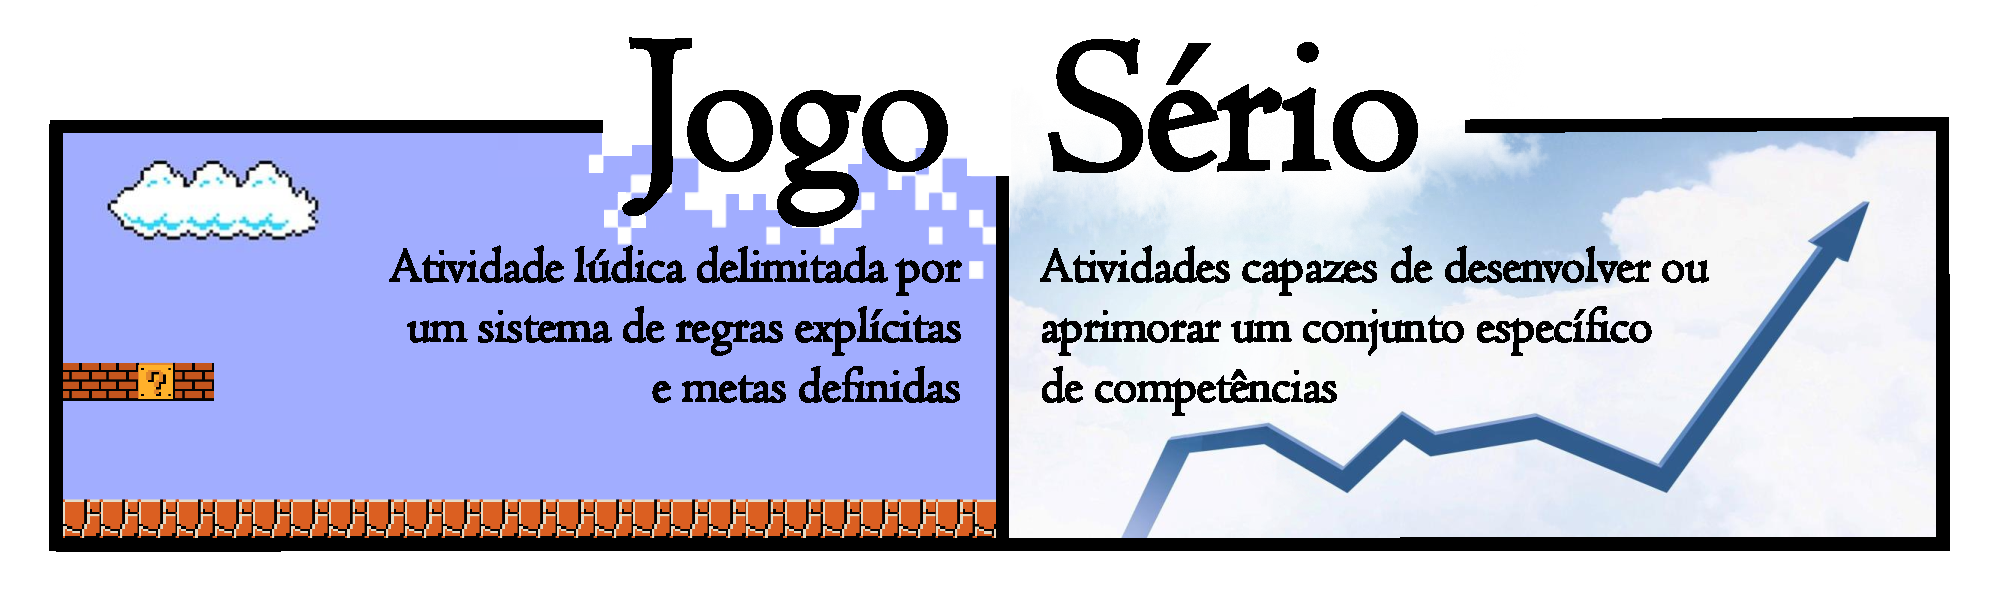
\includegraphics[width=\linewidth]{./Figuras/JogoSerio.pdf}
	\end{center} \vspace{-0,9cm}
  \legend{Fonte: os autores}

\end{figure}
%[GRAFICOOOOOO]http://downloads.hindawi.com/journals/ijcgt/2014/358152.pdf

\vspace{-0,4cm}

A Figura \ref{fig:JS} define separadamente a palavra \underline{Jo}g\underline{o} e \underline{Sério}. A união das definições dá o conceito de \underline{Jo}g\underline{o Sério} mais comum encontrado em pesquisas na área \cite{michael2005serious}. Enfatiza-se que para uma atividade se configurar como jogo, basta obeceder um conjunto de regras e objetivos. Um jogo nessa definição não precisa de quaisquer outros artefatos para se configurar como tal, podendo ainda, ocorrer individualmente ou coletivamente. Para um jogo abranger o caráter \underline{Sério} é necessário que o mesmo trabalhe em algum nível as habilidades físicas ou intelectuais de seus jogadores. 

\vspace{-0,1cm}

O aprimoramente ou desenvolvimento de habilidade físicas normalmente é associado aos \underline{Exer}g\underline{ames} \cite{araujo2017exergames, schroeder2017wobu}. Já o aprimoramente ou desenvolvimento de habilidade intelecutais é geralmente relacionado aos \underline{Jo}g\underline{os Educativos}. Pode-se dizer então que a classe de \underline{Jo}g\underline{o Sério} é uma generalização das áreas de \underline{Exer}g\underline{ames} e \underline{Jo}g\underline{os Educativos}. Salienta-se no entanto que para um jogo ser classificado como sério, não se faz necessário que o jogo compreenda ambas as áreas. Todavia, na definição mais aceita, um jogo sério deve abrager a área dos  \underline{Jo}g\underline{os Di}g\underline{itais} \cite{laamarti2014overview}.

%Outra área também associada aos jogos sérios é a área dos \underline{Jo}g\underline{os Di}g\underline{itais}.

\vspace{-0,1cm}

Os \underline{Jo}g\underline{os Di}g\underline{itais} são todo o conjunto de jogos, os quais são jogáveis apenas por intermédio de mídias digitais \cite{lucchese2009conceituaccao}. Os jogos digitais, englobam a definição clássica de \underline{Jo}g\underline{o}, necessitando também de um conjunto de regras e objetivos, porém acrescidos de um motor de jogo e uma interface interativa \cite{battaiola2000jogos}. Enquanto o motor de jogo fica responsável por controlar o conjunto de regras que rege o jogo. A interface interativa se encarrega de converter o jogo em si para sinais visuais e sonoros compreensíveis ao jogador.

\vspace{-0,1cm}

Os jogos digitais possuem um sistema de regras mais rigído em relação aos jogos clássicos, devido ao contexto computacional do motor de jogo. O mesmo contexto computacional também é responsável por trazer maior segurança aos jogos digitais em relação aos clássicos, uma vez que a interface interativa é capaz de contruir um ambiente lúdico inteiramente virtual, no qual os jogadores possam passar por situações de perigo sem que isso reflita em vias de fato em riscos aos jogadores \cite{lucchese2009conceituaccao}.

%http://www.dca.fee.unicamp.br/~martino/disciplinas/ia369/trabalhos/t1g3.pdf

%https://sci-hub.se/10.1109/MC.2005.297

Os jogos sérios assumem um importante papel no aprimoramento das habilidades de seus jogadores à medida que proprociam um ambiente seguro de interação. Ou seja, jogos sérios são jogos digitais porém projetados de modo que seus jogadores desenvolvam novas competências e/ou conhecimentos, ou reforcem capacidades existentes \cite{boller2017play}. O contexto digital de tais jogos ainda permite um sistema totalmente livre de julgamentos \cite{women2018international}. A depender a dinâmica do jogo, é possível que o jogador interaja com o ambiente virtual do jogo sem que seus erros tenham forte impacto no seu contexto social.

Os jogos sérios proporcionam um sistema de aprendizagem interativa. A aprendizagem interativa é um processo didático de ensino mais atrativo aos Nativos Digitais\footnote{Nativos Digitais é o termo ....Nativos Digitais é o termo ....Nativos Digitais é o termo ....Nativos Digitais é o termo ....Nativos Digitais é o termo ....Nativos Digitais é o termo ....Nativos Digitais é o termo ....}. Os nativos digitais apresentam maior preferencia por abordagens interativas baseadas em processos de tentativas e erro \cite{pescador2010tecnologias}. Além disso, os nativos digitais já nascem imersos no mundo digital, o que torna para eles, o processo de iteração com artefatos digitais, um processo mais natural e orgânico, em comparação a iteração entre tais artefatos e os Imigrantes Digitais\footnote{Imigrantes Digitais é o termo ....Imigrantes Digitais é o termo ....Imigrantes Digitais é o termo ....Imigrantes Digitais é o termo ....Imigrantes Digitais é o termo ....Imigrantes Digitais é o termo ....Imigrantes Digitais é o termo ....Imigrantes Digitais é o termo ....}.

%https://www.udesc.br/arquivos/cct/id_cpmenu/1024/diego_buchinger__1__15167055468902_1024.pdf [NATIVOS DIGITAIS]


Os jogos sérios manifestam-se como um facilitador no processo de apredizado dos nativos digitais. A abordagem de jogos sério no ambiente escolar podem trazer benefícios ao processo de ensino-aprendizagem, com efeito motivador, facilitador do aprendizado, desenvolvimento de habilidades cognitivas e aprendizado por descobertas \cite{de2017move4math}.

A literatura revela uma quantidade expressiva de aplicações para os jogos sérios, como as áreas da: saúde, educação, exército e mais \cite{zyda2005visual}. O presente estudo planeja o desenvolvimento de um jogo sério que há de compor um programa educacional para a prevenção da violência sexual infantil. A compreensão dos fundamentos que definem um jogo sério é indispensável para a progressão e conclusão deste trabalho. 

O presente trabalho baseia-se nos conceitos pesquisados e nas definições referenciadas nessa seção para fundamentar o jogo sério desenvolvido. Salienta-se que a estrutura lúdica e pedagógica do jogo são conceitos abordados por essa dissertação no Capítulo \ref{ch:Desenvolvimento}.




\newpage





%Ou seja, os nativos digitais apresentam maior predisposição pela busca e compreensão própria de determinados conceitos.




%Os nativos digitais preferem, num processo de tentativas e erro, ir se apropriando da lógica do programa ou do jogo, para utilizá-lo. Esse processo pode revelar uma forma de aprendizagem, que não é baseada em informações/instruções (que seria dada pelo manual), mas numa busca que parte daquele que precisa aprender, fuçar, explorar (a forma como o programa funciona).





%https://www.ucs.br/ucs/tplcinfe/eventos/cinfe/artigos/artigos/arquivos/eixo_tematico7/TECNOLOGIAS%20DIGITAIS%20E%20ACOES%20DE%20APRENDIZAGEM%20DOS%20NATIVOS%20DIGITAIS.pdf












%Salienta-se que a palavra \underline{Jo}g\underline{o} nessa definição não é sinônimo de \underline{brincadeira}, pois as brincadeiras de modo geral não assumem necessariamente um sistema de regras \cite{bertoldo2000jogar}.

%O termo \underline{Jo}g\underline{o Sério} (em inglês: \textit{Serious Game}) estabelece uma classe de jogos projetados para uma finalidade principal que não a pura diversão \cite{michael2005serious}. Sendo esta, a definição geral mais aceita, e identificada nas obras consultadas. 

%Por exemplo, explorar a aplicação de jogos para fins diferentes do entretenimento tem uma precedência histórica na aplicação do jogo - especialmente em contextos educacionais.

%Em outras palavras, são classificados desta forma, os jogos com propósitos sério, com o intuito de capacitar, educar ou aprimorar habilidades dos seus jogadores. 



%o Tavares (2007a) o entretenimento ´e utilizado com uma finalidade de passar conhecimentos, informa¸c˜oes, valores eatitudes.%https://files.cercomp.ufg.br/weby/up/498/o/Cuba2009.pdf
%Nesse enfoque e ainda com o que diz respeito a educa¸c˜ao, Tarouco et al. (2004) destaca que “os games podem se tornar ferramentas instrucionais eficientes, pois eles divertem e motivam, facilitando o aprendizado, pois aumenta a capacidade de reten¸c˜ao do que foi ensinado”.



%A classificação dos videogames está longe de ser uma nova ideia. Muitos sistemas de "classificações empíricas" já existem, e são realmente usados pela indústriade videogames, críticos e gamers. No entanto, mesmo que esses muitos sistemas sejam, sem dúvida, uma parte importante da cultura comum do videogame,eles infelizmente não são adequados para a classificação unificada de todos os videogames lançados. De fato, esses sistemas "empíricos" acompanham de perto a evolução dos videogames: novas categorias aparecem, outras são removidas, e suas definições continuam mudando, embora suas fronteiras permaneçam incertas.

%Além disso, não há um verdadeiro sistema de classificação geral reconhecido por todos: essas classificações são subjetivas e compartilhadas principalmente por pequenos grupos de usuários, para um conjunto definido de videogames.
%Várias tentativas de construir um sistema unificado a partir dessas classificações empíricas existem, mas nenhum desses sistemas baseados em acadêmicos ou de designers conseguiu produzir uma classificação reconhecida ainda... A partir dessa falta de classificação de videogame adequada para cada título lançado, levante a necessidade de explorar novas abordagens de classificação.





\section{Engenharia de Sotfware}\label{sec:Engenharia}

%\section{Learning Analytics}\label{sec:LA}


5) Game Design Document (GDD) [25]: É um documento guia do processo de desenvolvimento de um jogo e é dependente do contexto de cada projeto. O GDD precisa conter detalhes de jogabilidade, enredo, personagens, interface e regras do jogo. A falta dele pode ocasionar problemas sérios de design, falta de recursos e dificuldades de corrigir eventuais problemas [16]. %http://sbgames.org/sbgames2018/files/papers/ArtesDesignFull/188093.pdf


%1) Metodologia Maiêutica (M2 ) [22]: Apresenta uma proposta de metodologia de desenvolvimento de Ambientes Virtuais 3D Interativos com foco no processo de ensino e aprendizagem. O diferencial desta metodologia é a forma como ela conduz o processo de concepção, induzindo a reflexão e a criatividade.%http://sbgames.org/sbgames2018/files/papers/ArtesDesignFull/188093.pdf




%Avaliar a aprendizagem exige uma abordagem sistemática para determinar o sucesso e as dificuldades dos alunos (Bellotti et al., 2013). O grande desafio para criar essas avaliações é que necessitam naturalmente de serem tarefas do jogo, onde não se sacrifique a confiabilidade e validade do processo (Shute & Ke, 2012) e não se interrompa o fluxo na experiência de jogo correndo o risco do aluno perder o interesse (Chen, 2007). As interações com o jogo, ou seja, a sequência das ações, é que demonstram, com base nas escolhas do aluno, o que sabe ou não do assunto. O progresso do aluno ao avançar num jogo e acumular pontos de experiência pode ser uma evidência da sua aprendizagem. Não conseguir superar os desafios do jogo, representa que o aluno tem deficiências quanto às competências necessárias para fazê-lo, e rastrear as suas tentativas pode apontar quais são esses problemas e o apoio que necessita. Essas interações geram usualmente uma grande quantidade de dados a serem analisados. [tese ADILSON]

\section{Modelos Avaliativos}\label{sec:Engenharia}